\documentclass[11pt,letterpaper,twoside]{article}
\usepackage[english]{babel}
\usepackage{amssymb,amsmath}
\usepackage{fancyhdr}
\usepackage{graphicx}

 \oddsidemargin  0in \evensidemargin 0in
 \topmargin   -0.25in \headheight 0.25in \headsep 0.25in
 \textwidth   6.5in \textheight 8.75in \marginparsep 0pt \marginparwidth 0pt
 \parskip 1ex  \parindent 0ex \footskip 20pt

\newfont{\bssten}{cmssbx10}
\newfont{\bssnine}{cmssbx10 scaled 900}

%%%%%%%%%%%%%%%%%%%%%%%
\newcommand{\whatizit}{Lecture 10: Conditional Probability}
%%%%%%%%%%%%%%%%%%%%%%%


\pagestyle{fancy}  
\fancyhead{\bssnine STOR 155,  \whatizit}
\fancyhead[RE]{} \fancyhead[LO]{}
\fancyhead[LE]{\bssnine \thepage} \fancyhead[RO]{\bssnine \thepage}
\lfoot{} \cfoot{} \rfoot{}   


\newcommand{\var}{\mathrm{Var}}



\begin{document}



\thispagestyle{empty} \vspace*{-0.75in}

{\bssten STOR 155: Introduction to Data Models and Inference \hfill May 29, 2024 \\
Prof. Will Lassiter  \hfill Page 1 of \pageref{totalpag}}
\vspace{10pt}
\begin{center} {{\Large \bf \whatizit}} \end{center}

First example: student and parent drug use \vspace{-10pt}

\begin{center}
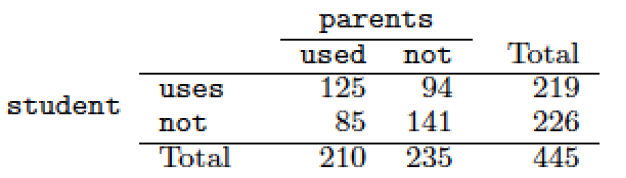
\includegraphics[scale=0.5]{images/druguse.png}
\end{center}

Random phenomenon: sample one student from this group and ask about drug use.

Venn diagram representation: \vspace{120pt}

\begin{itemize}

\item If the student tells us their parents use(d) drugs, what is the probability that they also use? \vspace{40pt}

\item If the student tells us they do not use drugs, what is the probability that their parents did/do? \vspace{40pt}

\end{itemize}

{\bf Terminology: Marginal and Joint Probabilities} \vspace{6pt}

{\bf Marginal} probability: \vspace{70pt}

{\bf Joint} probability: 

\newpage

Calculating marginal probabilities from joint probabilities: {\bf Law of Total Probability} \vspace{150pt}

{\bf Conditional Probability} \vspace{150pt}

\begin{center}
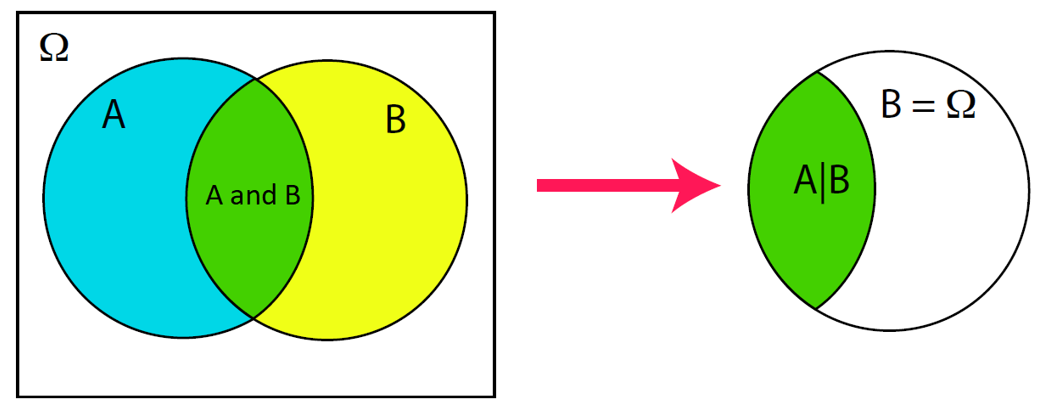
\includegraphics[scale=0.9]{images/conditional.png}
\end{center}

If events $A$ and $B$ are independent, then ...



\newpage

Example: Smallpox Outbreak in Boston, 1721 \vspace{-10pt}

\begin{center}
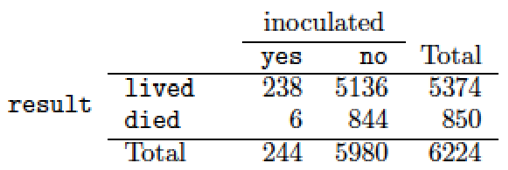
\includegraphics[scale=1]{images/smallpox.png}
\end{center}

Random phenomenon: sample one Bostonian's record and check how they fared during the outbreak

\begin{itemize}

\item What is the probability that they were not inoculated and died of smallpox? \vspace{30pt}

\item If they were not inoculated, what is the probability that they died of smallpox? \vspace{30pt}

\item If they were inoculated, what is the probability that they died of smallpox? \vspace{30pt}

\end{itemize}

Random phenomenon: Take a SRS of size 2 from Alice, Bob, Cindy, Dave, Eva \vspace{10pt}

Recall sample space: \vspace{10pt}

\begin{itemize}

\item $P(B)=$ \vspace{20pt}

\item $P(B|A)=$ \vspace{40pt}

\end{itemize}

{\bf General Multiplication Rule} \vspace{70pt} 

Example: Suppose we are given only two
pieces of information from the smallpox data: 96.08\% of residents were not inoculated, and 85.88\% of the residents who were not inoculated ended up surviving. How could we compute the probability that a resident was not inoculated and survived? 


\newpage

Rules for conditional probabilities:

\begin{itemize}

\item If $A$ and $B$ are disjoint events and $C$ is another event, \vspace{30pt}

\item For any two events $A$ and $B$, \vspace{30pt}

\end{itemize}

Working off of the previous question, what is the probability that a randomly chosen resident died given they were not inoculated? \vspace{40pt}

{\bf Bayes' Theorem}

Random phenomenon: Flip a fair coin to determine which jar (heads = jar 1, tails = jar 2) we will draw a colored ball from without looking and record the color of the ball that is drawn.

\begin{center}
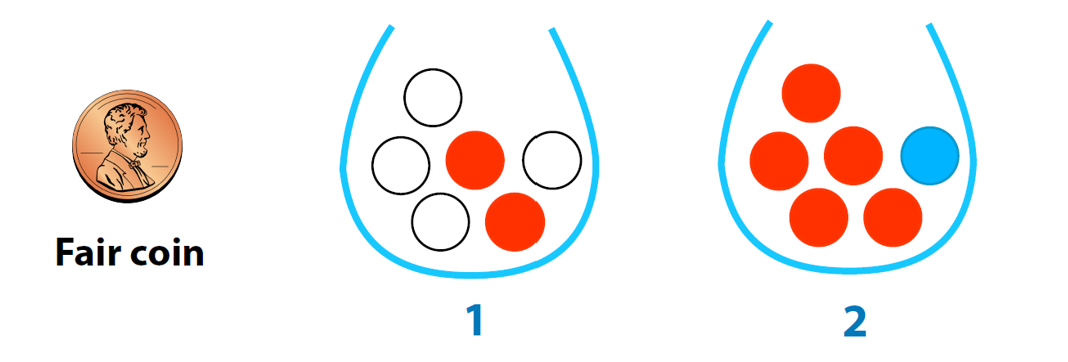
\includegraphics[scale=1]{images/bayes.png}
\end{center}

Sample space? \vspace{20pt}

Working out probabilities for each outcome: probability tree

\newpage

Given that we drew a red ball, what is the probability that the coin flip came up heads? \vspace{200pt}

Bayes' Theorem: general form \vspace{150pt}

Example: Monty Hall Problem

You're on a game show where you're given the choice of three doors: Behind one door is a car; behind the others, goats (obviously you want the car). You start the game by choosing a door, say door number 1.  To make things interesting, the host, who knows what's behind each door, opens one of the doors you didn't choose, say door number 3, revealing a goat. He then asks, ``Do you want to switch your choice to door number 2, or stick with door number 1?" What should you do?

\newpage

Practice: Spam-B-Gone is a computer application that learns to sort e-mail into 3 distinct categories --- high-priority ({\bf H}), low-priority ({\bf L}), or spam ({\bf S}) --- based on feedback collected from a user over a week-long trial period. During Bill's trial period, he received a total of 1200 e-mails and labeled 200 of them as {\bf H}, 600 as {\bf L}, and 400 as {\bf S}.  Spam-B-Gone now hopes to use Bill's feedback to automatically classify all future e-mails he receives.

One of Spam-B-Gone's classification methods involves scanning for certain keywords, e.g.\ ``offer", that are more likely to show up in spam e-mails. In Bill's case, just 4 of the 200 e-mails he labeled {\bf H} included the word ``offer", while 30 of the 600 {\bf L} e-mails and 320 of the 400 {\bf S} emails included ``offer".

\begin{itemize}

\item If all Bill's future e-mails follow the same distribution as we observed during the trial period, what is the probability that the next e-mail Bill receives is not spam? \vspace{40pt}

\item What is the probability that the next e-mail Bill receives includes the word ``offer"? \vspace{40pt}

\item Given that the next e-mail Bill receives includes the word ``offer", what is the probability that he would classify it as a spam e-mail?

\end{itemize}

\label{totalpag}
\end{document}